% Template for PLoS
% Version 3.5 March 2018
%
% % % % % % % % % % % % % % % % % % % % % %
%
% -- IMPORTANT NOTE
%
% This template contains comments intended
% to minimize problems and delays during our production
% process. Please follow the template instructions
% whenever possible.
%
% % % % % % % % % % % % % % % % % % % % % % %
%
% Once your paper is accepted for publication,
% PLEASE REMOVE ALL TRACKED CHANGES in this file
% and leave only the final text of your manuscript.
% PLOS recommends the use of latexdiff to track changes during review, as this will help to maintain a clean tex file.
% Visit https://www.ctan.org/pkg/latexdiff?lang=en for info or contact us at latex@plos.org.
%
%
% There are no restrictions on package use within the LaTeX files except that
% no packages listed in the template may be deleted.
%
% Please do not include colors or graphics in the text.
%
% The manuscript LaTeX source should be contained within a single file (do not use \input, \externaldocument, or similar commands).
%
% % % % % % % % % % % % % % % % % % % % % % %
%
% -- FIGURES AND TABLES
%
% Please include tables/figure captions directly after the paragraph where they are first cited in the text.
%
% DO NOT INCLUDE GRAPHICS IN YOUR MANUSCRIPT
% - Figures should be uploaded separately from your manuscript file.
% - Figures generated using LaTeX should be extracted and removed from the PDF before submission.
% - Figures containing multiple panels/subfigures must be combined into one image file before submission.
% For figure citations, please use "Fig" instead of "Figure".
% See http://journals.plos.org/plosone/s/figures for PLOS figure guidelines.
%
% Tables should be cell-based and may not contain:
% - spacing/line breaks within cells to alter layout or alignment
% - do not nest tabular environments (no tabular environments within tabular environments)
% - no graphics or colored text (cell background color/shading OK)
% See http://journals.plos.org/plosone/s/tables for table guidelines.
%
% For tables that exceed the width of the text column, use the adjustwidth environment as illustrated in the example table in text below.
%
% % % % % % % % % % % % % % % % % % % % % % % %
%
% -- EQUATIONS, MATH SYMBOLS, SUBSCRIPTS, AND SUPERSCRIPTS
%
% IMPORTANT
% Below are a few tips to help format your equations and other special characters according to our specifications. For more tips to help reduce the possibility of formatting errors during conversion, please see our LaTeX guidelines at http://journals.plos.org/plosone/s/latex
%
% For inline equations, please be sure to include all portions of an equation in the math environment.
%
% Do not include text that is not math in the math environment.
%
% Please add line breaks to long display equations when possible in order to fit size of the column.
%
% For inline equations, please do not include punctuation (commas, etc) within the math environment unless this is part of the equation.
%
% When adding superscript or subscripts outside of brackets/braces, please group using {}.
%
% Do not use \cal for caligraphic font.  Instead, use \mathcal{}
%
% % % % % % % % % % % % % % % % % % % % % % % %
%
% Please contact latex@plos.org with any questions.
%
% % % % % % % % % % % % % % % % % % % % % % % %

\documentclass[10pt,letterpaper]{article}
\usepackage[top=0.85in,left=2.75in,footskip=0.75in]{geometry}

% amsmath and amssymb packages, useful for mathematical formulas and symbols
\usepackage{amsmath,amssymb}

% Use adjustwidth environment to exceed column width (see example table in text)
\usepackage{changepage}

% Use Unicode characters when possible
\usepackage[utf8x]{inputenc}

% textcomp package and marvosym package for additional characters
\usepackage{textcomp,marvosym}

% cite package, to clean up citations in the main text. Do not remove.
% \usepackage{cite}

% Use nameref to cite supporting information files (see Supporting Information section for more info)
\usepackage{nameref,hyperref}

% line numbers
\usepackage[right]{lineno}

% ligatures disabled
\usepackage{microtype}
\DisableLigatures[f]{encoding = *, family = * }

% color can be used to apply background shading to table cells only
\usepackage[table]{xcolor}

% array package and thick rules for tables
\usepackage{array}

% create "+" rule type for thick vertical lines
\newcolumntype{+}{!{\vrule width 2pt}}

% create \thickcline for thick horizontal lines of variable length
\newlength\savedwidth
\newcommand\thickcline[1]{%
  \noalign{\global\savedwidth\arrayrulewidth\global\arrayrulewidth 2pt}%
  \cline{#1}%
  \noalign{\vskip\arrayrulewidth}%
  \noalign{\global\arrayrulewidth\savedwidth}%
}

% \thickhline command for thick horizontal lines that span the table
\newcommand\thickhline{\noalign{\global\savedwidth\arrayrulewidth\global\arrayrulewidth 2pt}%
\hline
\noalign{\global\arrayrulewidth\savedwidth}}


% Remove comment for double spacing
%\usepackage{setspace}
%\doublespacing

% Text layout
\raggedright
\setlength{\parindent}{0.5cm}
\textwidth 5.25in
\textheight 8.75in

% Bold the 'Figure #' in the caption and separate it from the title/caption with a period
% Captions will be left justified
\usepackage[aboveskip=1pt,labelfont=bf,labelsep=period,justification=raggedright,singlelinecheck=off]{caption}
\renewcommand{\figurename}{Fig}

% Use the PLoS provided BiBTeX style
% \bibliographystyle{plos2015}

% Remove brackets from numbering in List of References
\makeatletter
\renewcommand{\@biblabel}[1]{\quad#1.}
\makeatother



% Header and Footer with logo
\usepackage{lastpage,fancyhdr,graphicx}
\usepackage{epstopdf}
%\pagestyle{myheadings}
\pagestyle{fancy}
\fancyhf{}
%\setlength{\headheight}{27.023pt}
%\lhead{
\includegraphics[width=2.0in]{PLOS-submission.eps}}
\rfoot{\thepage/\pageref{LastPage}}
\renewcommand{\headrulewidth}{0pt}
\renewcommand{\footrule}{\hrule height 2pt \vspace{2mm}}
\fancyheadoffset[L]{2.25in}
\fancyfootoffset[L]{2.25in}
\lfoot{\today}

%% Include all macros below

\newcommand{\lorem}{{\bf LOREM}}
\newcommand{\ipsum}{{\bf IPSUM}}


% Pandoc citation processing

\usepackage{float} \floatplacement{figure}{H} \usepackage{float} \floatplacement{figure}{H} \newcommand{\beginsupplement}{\setcounter{table}{0} \renewcommand{\thetable}{S\arabic{table}} \setcounter{figure}{0} \renewcommand{\thefigure}{S\arabic{figure}}}
\usepackage{booktabs}
\usepackage{longtable}
\usepackage{array}
\usepackage{multirow}
\usepackage{wrapfig}
\usepackage{float}
\usepackage{colortbl}
\usepackage{pdflscape}
\usepackage{tabu}
\usepackage{threeparttable}
\usepackage{threeparttablex}
\usepackage[normalem]{ulem}
\usepackage{makecell}
\usepackage{xcolor}



\usepackage{forarray}
\usepackage{xstring}
\newcommand{\getIndex}[2]{
  \ForEach{,}{\IfEq{#1}{\thislevelitem}{\number\thislevelcount\ExitForEach}{}}{#2}
}

\setcounter{secnumdepth}{0}

\newcommand{\getAff}[1]{
  \getIndex{#1}{}
}

\providecommand{\tightlist}{%
  \setlength{\itemsep}{0pt}\setlength{\parskip}{0pt}}

\begin{document}
\vspace*{0.2in}

% Title must be 250 characters or less.
\begin{flushleft}
{\Large
\textbf\newline{Short-term forecasting of total Number of reported COVID-19 cases in
South Africa - A Bayesian temporal modeling approch} % Please use "sentence case" for title and headings (capitalize only the first word in a title (or heading), the first word in a subtitle (or subheading), and any proper nouns).
}
\newline
% Insert author names, affiliations and corresponding author email (do not include titles, positions, or degrees).
\\
Belay Birlie Yimer\textsuperscript{\getAff{Arthritis Research UK Centre for Epidemiology, Division of
Musculoskeletal and Dermatological Sciences, The University of
Manchester, Manchester;}, \getAff{Interuniversity Institute for Biostatistics and statistical
Bioinformatics (I-BioStat), Hasselt University, Diepenbeek, Belgium.}},
Ziv Shkedy\textsuperscript{\getAff{Interuniversity Institute for Biostatistics and statistical
Bioinformatics (I-BioStat), Hasselt University, Diepenbeek, Belgium.}}\\
\bigskip
\bigskip
\end{flushleft}
% Please keep the abstract below 300 words
\section*{Abstract}
To be updated.

% Please keep the Author Summary between 150 and 200 words
% Use first person. PLOS ONE authors please skip this step.
% Author Summary not valid for PLOS ONE submissions.
\section*{Author summary}
To be updated.

\linenumbers

% Use "Eq" instead of "Equation" for equation citations.
\hypertarget{introduction}{%
\section{Introduction}\label{introduction}}

In this paper we present (1) South Africa's COVID trajectory to the
first 100,000 (22 June 2020) cases and (2) fit a series of non-linear
growth models, calibrated to COVID-19 cumulative number of reported case
data from 5 March 2020 to 22 June 2020. The models are used to produce
short term predictions of the number of reported cases expected for a
period of 30 days ahead. These forecasts are generated at the national
level

\hypertarget{methods}{%
\section{Methods}\label{methods}}

\hypertarget{data}{%
\subsection{Data}\label{data}}

We downloaded data from Coronavirus COVID-19 (2019-nCoV) Data Repository
for South Africa maintained by Data Science for Social Impact research
group at the University of Pretoria {[}ref{]}. The data repository
captures the daily number of new cases, number of tests, number of
deaths and recoveries. Our primary outcome of interest was the daily
number of newly diagnosed COVID-19 cases and the unit of time used in
modelling was a day. We used the daily case reports from March 12, 2020,
until February 27, 2021, in our analysis.

\hypertarget{statistical-analysis}{%
\subsection{Statistical analysis}\label{statistical-analysis}}

We considered two widely used temporal models to model the daily number
of newly diagnosed COVID-19 cases. We let \(Y(t)\) denote the daily
number of newly diagnosed COVID-19 cases at time \(t\) and \(\mu(t)\)
represent the expected number of cases at time \(t\). We considered a
Negative binomial distribution for \(Y(t)\) to account for possible
overdispersion. That is, \(Y(t) \sim NB(\mu(t), \delta)\), where
\(\delta\) is the overdispersion parameter. We considered two temporal
models to capture the trend over time: a random walk of order two
(\(RW(2)\)) and an autoregressive model of order one (\(AR(1)\))
{[}1{]}. We also considerd a \(RW(1)\) model, but the model overfits the
data (See the supplemntary appendix). Similarly, we considerd an \(AR\)
model order \(p=2\) but the result is similar to \(AR1\) model and we
prefer the simpler \(AR1\) model.

The \(AR(1)\) model {[}1{]} is given by,

\[
\begin{aligned}
 Y(t) &\sim NB(\mu(t), \delta) \ \ t=1, \dots, n,\\
 log(\mu(t)) &= \alpha+u_t, \\
 u_1 &\sim N(0, \tau_u(1-\rho^2)^{-1}),  \\
  u_t &=\rho u_{t-1} +\epsilon_t, \ \ t=2, \dots, n,  \\
  \epsilon_t & \sim N(0, \tau_{\epsilon}),
\end{aligned}
\] where, \(\alpha\) is an intercept, \(\rho\) a temporal correlation
term (with \(|\rho|<1\)) and \(\epsilon_t\) is a Gaussian error term
with zero mean and precision \(\tau_{\epsilon}\).

Similarly, the \(RW(2)\) model {[}1{]} is given by, \[
\begin{aligned}
 Y(t) &\sim NB(\mu(t), \delta) \ \ t=1, \dots, n,\\
 log(\mu(t)) &= \alpha+u_t, \\
 u_t-2u_{t+1}+u_{t+2} &\sim N(0, \tau_u), \ \ t=2, \dots, n,
\end{aligned}
\] where \(\alpha\) is the intercept term as before and \(\tau_u\) is
the precison parameter.

The two models were fitted within the Bayesian framework using
\emph{inla} {[}2{]}. To complete the specification of both models, we
assume the following priors. For the \(AR(1)\) model, we denote
\(\theta_1=log(\tau_u(1-\rho^2))\) where \(\Gamma(10,100)\) prior is
specified for \(\theta_1\), and we denote
\(\theta_2=log\frac{1+\rho}{1-\rho}\) and assume a \(N(0, 0.15)\) prior
for \(\theta\). Similarly, we represent the precison parameter of
\(RW(1)\), \(\tau_u\), as \(\theta=log(\tau_u)\) and assume a
\(\Gamma (10,100)\) prior for \(\theta\).

To assess the models' accuracy in predicting COVID-19 cases, we present
the forecast period's actual observed values and the predicted values.
Additionally, the model fits were evaluated by using DIC (Deviance
information criteria).

The R-code that we used for our analyses is avaliable at
https://github.com/belayb/COVIDincidenceSA/tree/master/COVIDincidenceSA.

\hypertarget{results}{%
\section{Results}\label{results}}

The daily number of reported COVID-19 cases from 12
March 2020 to 27 February 2021 is presented in Figure \ref{fig:daily-cases}. Similar to elsewhere in the world, South
Africa pass through a two-wave pandemic. The pandemic first peak was
on 07 July 2020, where up to 13944 new COVID-19 cases reported, followed
by a second peak in January 2021, where more than 21,000 daily cases
reported. Figure \ref{fig:cummulative} presents the cumulative number of reported
COVID-19 cases and tests performed. To date, 8,838,937 tests have been
conducted, and a total of 1,500,677 cases reported.

\begin{figure}[H]
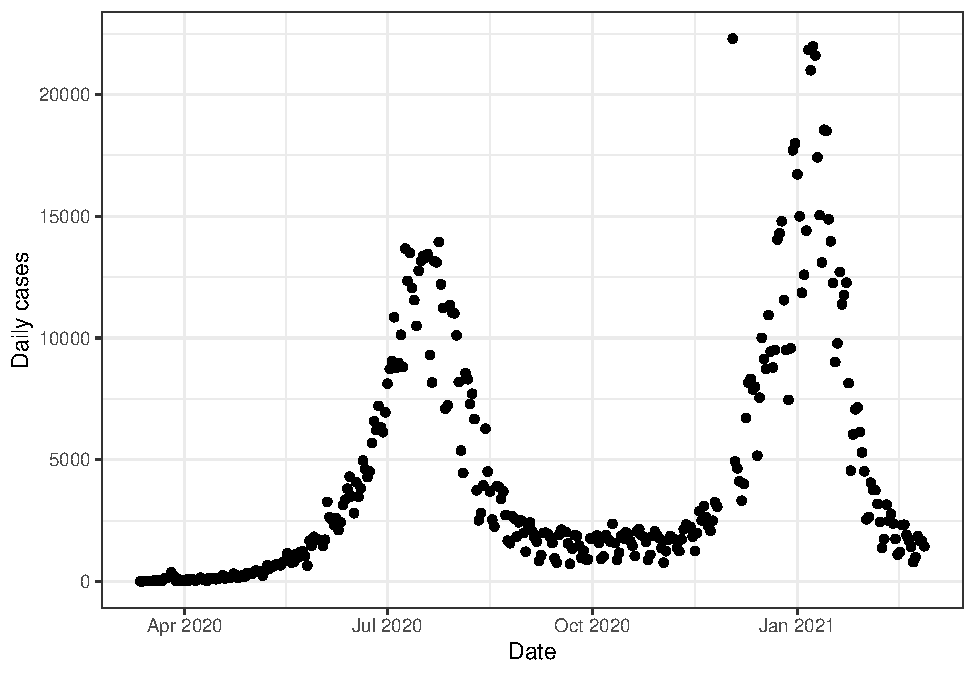
\includegraphics[width=0.99\linewidth]{COVIDincidenceSA_files/figure-latex/daily-cases-1} \caption{Daily number of COVID-19 cases in South Africa from 12/03/2020-27/02/2021.}\label{fig:daily-cases}
\end{figure}

\begin{figure}[H]
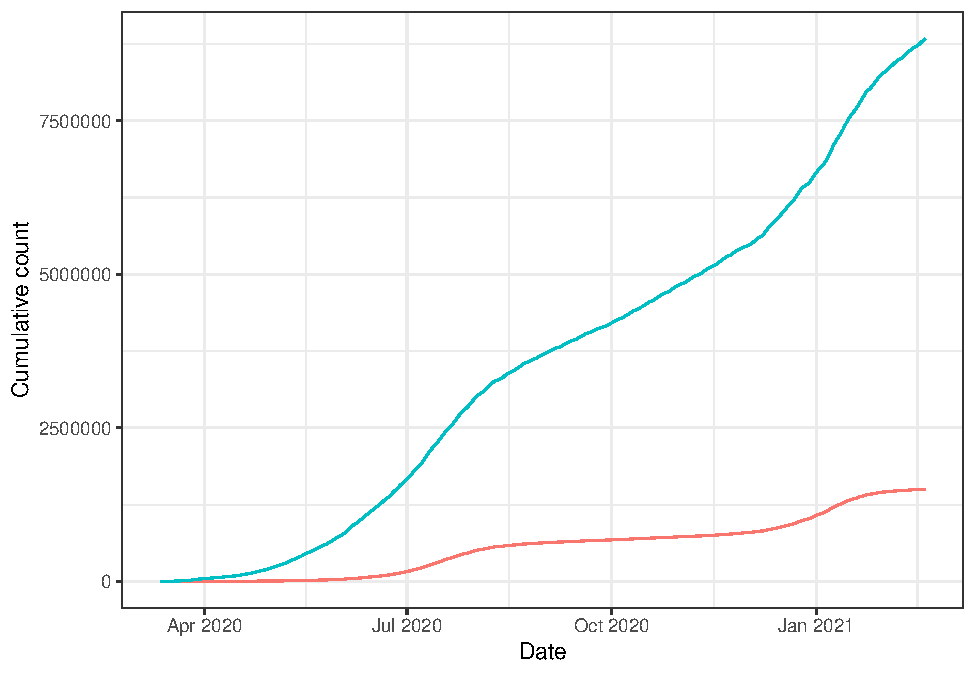
\includegraphics[width=0.99\linewidth]{COVIDincidenceSA_files/figure-latex/cummulative-1} \caption{The cummulative number of COVID-19 cases and Cummulative number of tests in South Africa from 12/03/2020-27/02/2021. Red-line denote the number of cases and blue-line denotes the number of tests.}\label{fig:cummulative}
\end{figure}

\hypertarget{short-term-prediction-of-the-total-number-of-reported-covid-19-cases}{%
\subsection{Short-term prediction of the total number of reported
COVID-19
cases}\label{short-term-prediction-of-the-total-number-of-reported-covid-19-cases}}

We fit the four models models described in the previous section to the daily
reported new COVID-19 cases. The parameter estimates for the two models
are presented in Supplementary Table 1. As depicted in Figure 3, two
models fitted to the data appear to fit the observed data (within the
estimation period) well with a narrow confidence interval obtained for
the \(RW(2)\) model. The two models provides similar predictions over
the 7-day ahead period.



\begin{table}[!h]
	
	\caption{\label{tab:Accuracy}Accuracy metrics of forecasting for AR1, AR2, RW1, and RW2 models.}
	\centering
	\begin{tabular}[t]{lrrrr}
		\hline
		Days ahead point forecasts & \multicolumn{4}{c}{Mean Absolute Error}\\
		\cline{2-5}
		& RW1 & RW2 & AR1 & AR2\\
		\hline
		One day & 449.2918 & 3482.401 & 1201.786 & 1056.635\\
		\hline
		Two day & 1308.8048 & 3575.291 & 1871.106 & 1716.237\\
		\hline
		Three day & 2351.2483 & 3758.596 & 2777.020 & 2636.543\\
		\hline
		Four day & 3327.8508 & 3890.326 & 3620.173 & 3460.322\\
		\hline
		Five day & 4227.1623 & 3951.276 & 4348.963 & 4164.685\\
		\hline
		Six day & 4982.3087 & 3909.428 & 4893.645 & 4679.546\\
		\hline
		Seven day & 5821.8832 & 3959.609 & 5479.801 & 5230.147\\
		\hline\\
		& \multicolumn{4}{c}{Mean Absolute Percentage Error}\\
		\cline{2-5}\\
		& RW1 & RW2 & AR1 & AR2\\
		\hline\\
		One day & 0.0003005 & 0.0023281 & 0.0008036 & 0.0007065\\
		\hline
		Two day & 0.0008742 & 0.0023875 & 0.0012498 & 0.0011463\\
		\hline
		Three day & 0.0015690 & 0.0025074 & 0.0018531 & 0.0017593\\
		\hline
		Four day & 0.0022186 & 0.0025927 & 0.0024135 & 0.0023069\\
		\hline
		Five day & 0.0028151 & 0.0026302 & 0.0028962 & 0.0027734\\
		\hline
		Six day & 0.0033140 & 0.0025989 & 0.0032550 & 0.0031125\\
		\hline
		Seven day & 0.0038681 & 0.0026291 & 0.0036407 & 0.0034748\\
		\hline\\
		& \multicolumn{4}{c}{Information Criteria}\\
		\hline\\
		DIC & 5059.06 & 5447.40 & 5278.87 & 5284.00\\
		WAIC & 5123.56 & 5460.81 & 5286.90 & 5294.74\\
		\hline\\
	\end{tabular}
\end{table}

\begin{figure}[H]
	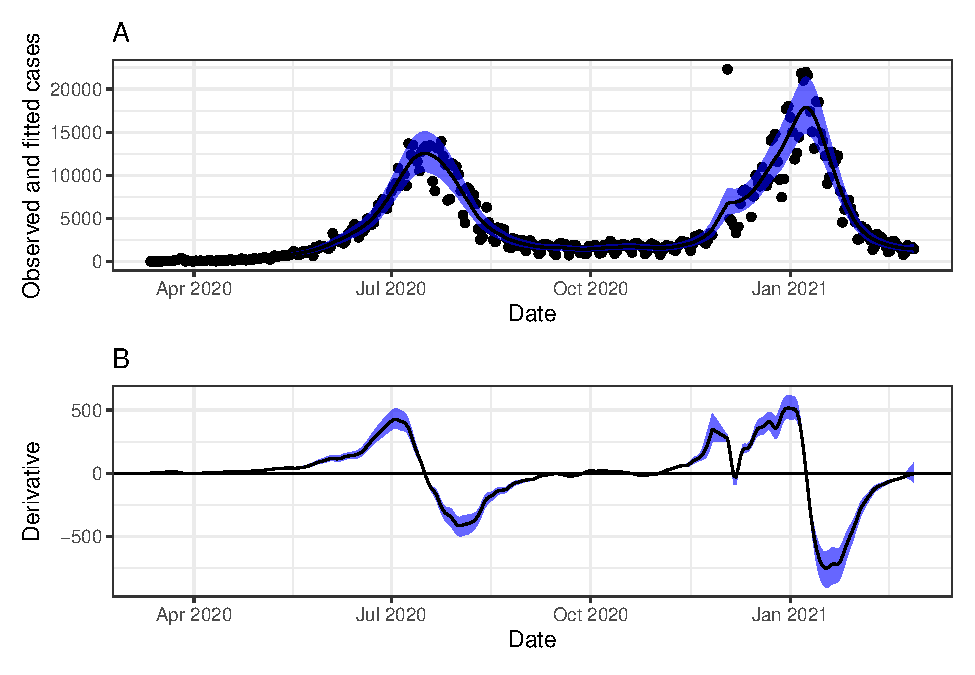
\includegraphics[width=0.95\linewidth]{COVIDincidenceSA_files/figure-latex/unnamed-chunk-7-1} \caption{RW2 model for the daily confirmed COVID-19 cases in South Africa 12/03/2020-27/02/2021.  Panel A-fitted and observed data. The balck dotes are the observed number of daily cases, the black solid line the fitted curve, and the blue shaded area is the 95\% credible interval. Panel B-first-order derivative of the fitted curve along with the 95\% credible interval.}\label{fig:unnamed-chunk-7}
\end{figure}


\begin{figure}[H]
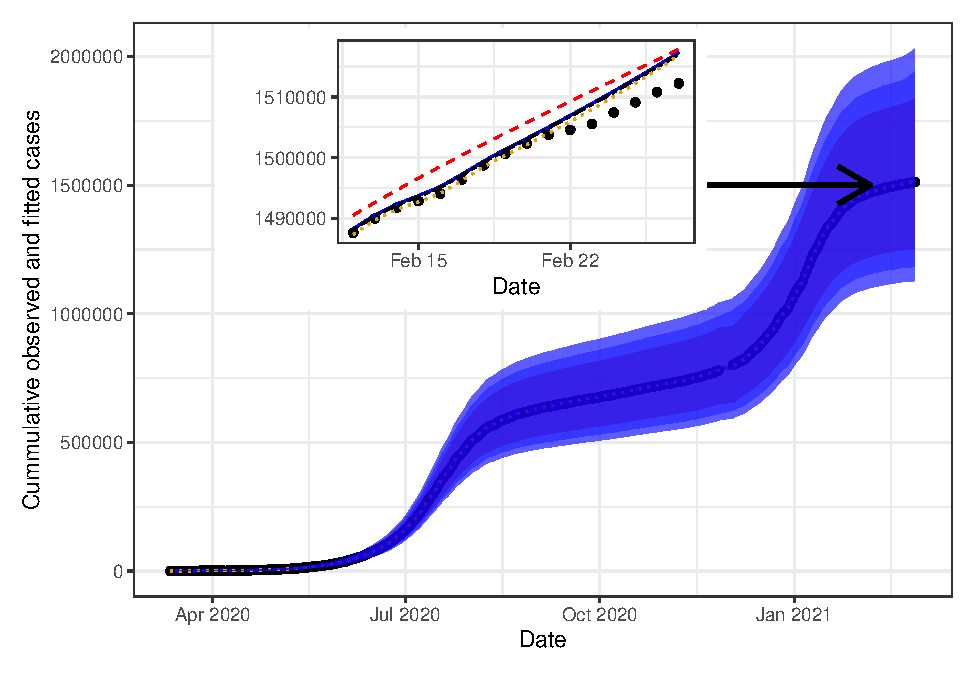
\includegraphics[width=0.95\linewidth]{COVIDincidenceSA_files/figure-latex/predd-1} \caption{Predicted cummulative COVID-19 cases in South Africa under the RW(1) and AR(1) model. Estimation period 12/03/2020-20/02/2021. The black dots are the observed cummulative cases. The red dashed lines are for RW(2) and the blue line for AR(1).The shaded bands are the prediction intervals. }\label{fig:predd}
\end{figure}

\begin{table}[!h]

\caption{\label{tab:unnamed-chunk-10}Short-term predictions of total number of reported cases at the national level under the rw2 model. Estimation period 12/03/2020-20/02/2021}
\centering
\begin{tabular}[t]{l|r|r|l|r}
\hline
Date & Total & Prediction & Prediction Interval & Total - Prediction\\
\hline
2021-02-21 & 1503796 & 1507571 & (1248627.38-1814985.53) & -3774.603\\
\hline
2021-02-22 & 1504588 & 1509293 & (1249674.84-1817725.91) & -4704.805\\
\hline
2021-02-23 & 1505586 & 1511002 & (1250614.44-1820669.35) & -5415.664\\
\hline
2021-02-24 & 1507448 & 1512704 & (1251450.03-1823858.23) & -5255.522\\
\hline
2021-02-25 & 1509124 & 1514405 & (1252187.39-1827339.44) & -5281.407\\
\hline
2021-02-26 & 1510778 & 1516115 & (1252833.56-1831166.58) & -5337.172\\
\hline
2021-02-27 & 1512225 & 1517842 & (1253396.63-1835400.97) & -5616.650\\
\hline
\end{tabular}
\end{table}

\begin{table}[!h]

\caption{\label{tab:unnamed-chunk-10}Short-term predictions of total number of reported cases at the national level under the AR1 model. Estimation period 12/03/2020-20/02/2021}
\centering
\begin{tabular}[t]{l|r|r|l|r}
\hline
Date & Total & Prediction & Prediction Interval & Total - Prediction\\
\hline
2021-02-21 & 1503796 & 1505071 & (1124486.84-1998035.3) & -1274.995\\
\hline
2021-02-22 & 1504588 & 1506982 & (1125286.9-2001911.8) & -2393.764\\
\hline
2021-02-23 & 1505586 & 1508942 & (1125972.18-2006363.99) & -3356.174\\
\hline
2021-02-24 & 1507448 & 1510953 & (1126572.19-2011372.04) & -3504.598\\
\hline
2021-02-25 & 1509124 & 1513014 & (1127105.33-2016924.89) & -3889.609\\
\hline
2021-02-26 & 1510778 & 1515126 & (1127584.21-2023016.99) & -4347.854\\
\hline
2021-02-27 & 1512225 & 1517290 & (1128017.98-2029646.04) & -5065.020\\
\hline
\end{tabular}
\end{table}









\newpage

\hypertarget{appendix}{%
\section{Appendix}\label{appendix}}

\setcounter{table}{0} \renewcommand{\thetable}{S\arabic{table}} \setcounter{figure}{0} \renewcommand{\thefigure}{S\arabic{figure}}

\begin{figure}[H]
	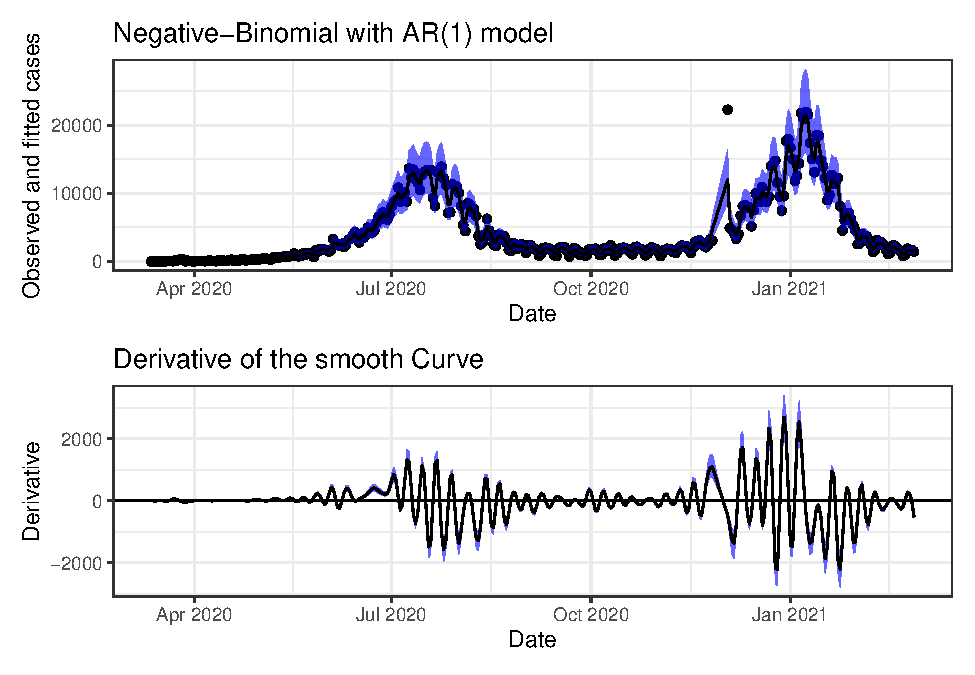
\includegraphics[width=0.99\linewidth]{COVIDincidenceSA_files/figure-latex/unnamed-chunk-6-1} \caption{Fitted and observed data AR(1) model}\label{fig:unnamed-chunk-6}
\end{figure}

\begin{figure}[H]
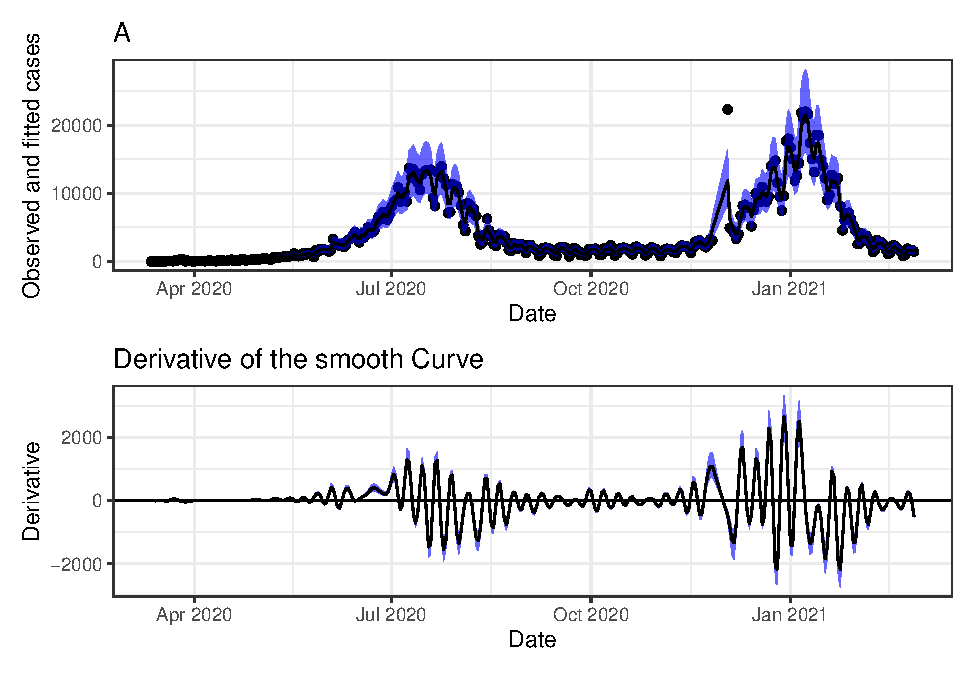
\includegraphics[width=0.99\linewidth]{COVIDincidenceSA_files/figure-latex/unnamed-chunk-13-1} \caption{Fitted and observed data AR(2) model}\label{fig:unnamed-chunk-13}
\end{figure}

\begin{figure}[H]
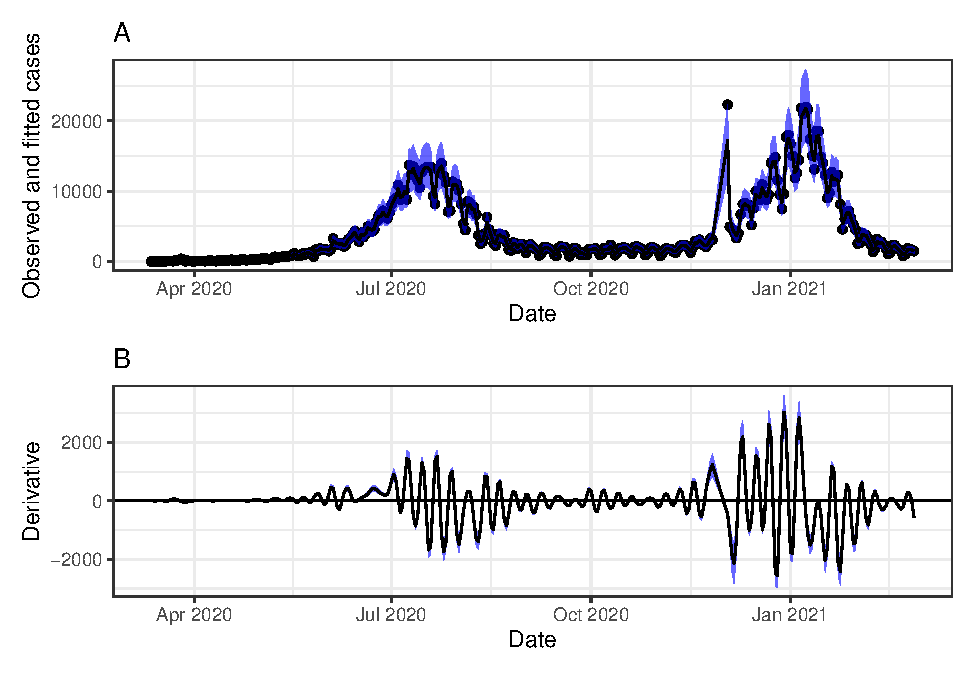
\includegraphics[width=0.99\linewidth]{COVIDincidenceSA_files/figure-latex/unnamed-chunk-14-1} \caption{Fitted and observed data RW(1) model}\label{fig:unnamed-chunk-14}
\end{figure}

\begin{table}[!h]
	
	\caption{\label{tab:unnamed-chunk-11}Parameter estimates AR1 model}
	\centering
	\begin{tabular}[t]{l|r|r|r|r}
		\hline
		& mean & sd & 0.025quant & 0.975quant\\
		\hline
		(Intercept) & 6.109 & 2.441 & 0.145 & 10.569\\
		\hline
		Size & 28.955 & 8.389 & 16.805 & 49.397\\
		\hline
		Precision for time & 0.158 & 0.112 & 0.023 & 0.438\\
		\hline
		Rho for time & 0.995 & 0.004 & 0.985 & 0.999\\
		\hline
	\end{tabular}
\end{table}

\begin{table}[!h]
	
	\caption{\label{tab:unnamed-chunk-11}Parameter estimates RW2 model}
	\centering
	\begin{tabular}[t]{l|r|r|r|r}
		\hline
		& mean & sd & 0.025quant & 0.975quant\\
		\hline
		(Intercept) & 7.603 & 0.017 & 7.570 & 7.637\\
		\hline
		Size & 10.422 & 0.911 & 8.734 & 12.319\\
		\hline
		Precision for time & 0.036 & 0.014 & 0.016 & 0.070\\
		\hline
	\end{tabular}
\end{table}

\begin{figure}[H]
	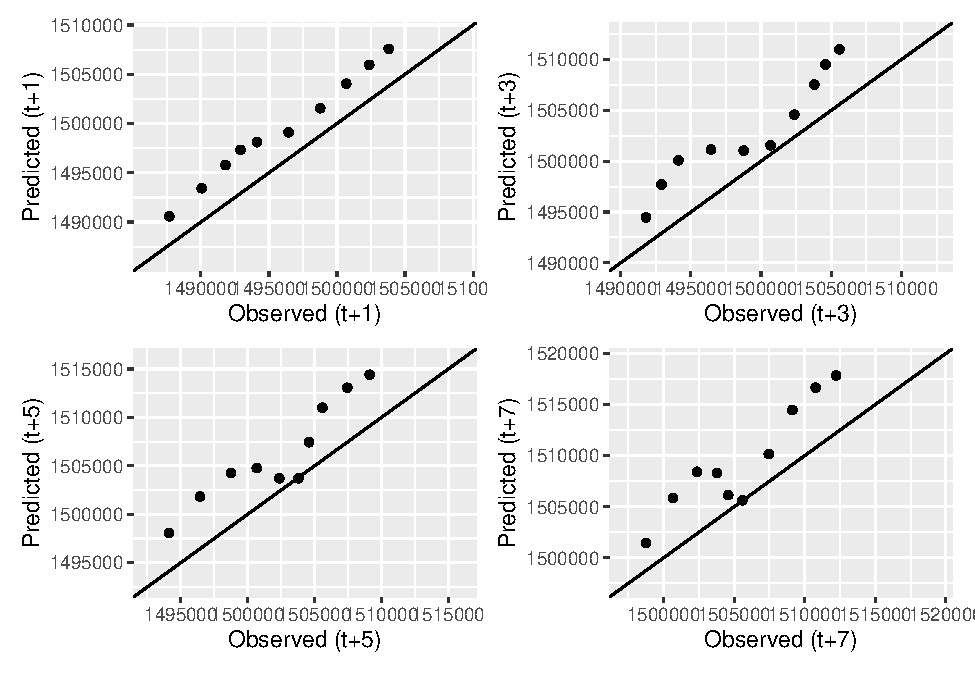
\includegraphics[width=0.99\linewidth]{COVIDincidenceSA_files/figure-latex/accuracy-1} \caption{Predicted vs observed cummulative COVID-19 cases in South Africa under the RW(2) model. Base estimation period 12/03/2020-10/02/2021. The estimation period was expanded by 1 day until 20/02/2021}\label{fig:accuracy}
\end{figure}

\hypertarget{references}{%
\section*{References}\label{references}}
\addcontentsline{toc}{section}{References}

\hypertarget{refs}{}
\leavevmode\hypertarget{ref-gomez2020bayesian}{}%
1. Gómez-Rubio V. Bayesian inference with inla. CRC Press; 2020.

\leavevmode\hypertarget{ref-martins2013bayesian}{}%
2. Martins TG, Simpson D, Lindgren F, Rue H. Bayesian computing with
inla: New features. Computational Statistics \& Data Analysis. Elsevier;
2013;67: 68--83.

\nolinenumbers


\end{document}

